\section{Missing transverse energy}\label{sec:met}

In hadron colliders the longitudinal momentum (along the beam axis) carried by the incoming partons is not known, preventing the possibility to measure the total missing energy. Nevertheless, the initial transverse momentum carried by the incoming partons is expected to be practically zero, thereby, for the conservation of the momentum components, also the net momentum of all the particles in the final state of collisions must be zero. The missing transverse momentum (\ptmiss) is the momentum imbalance in the transverse plane of all the visible particles in the event, and its modulus is the missing transverse energy (\MET). The \ptmiss vector is defined as the negative vectorial sum of transverse momenta of all reconstructed PF objects, as shown in the following equation:
\begin{equation}\label{eq:met}
\ptmiss = - \sum_{\mathrm{PF\,obj}} \vec{p}_\mathrm{T}^\mathrm{\,PF\,obj} \quad,
\end{equation}

\noindent where the sum extends over all the PF objects.
A value of \MET different from zero is a potential signature of the presence of particles in the event that have not interacted with the detector, such as neutrinos or particles predicted by some BSM models. Nevertheless, the presence of \MET in the event can also be ascribed to detector inefficiencies.

In addition to imperfect resolution of all detectable and reconstructed physics objects, the \MET measurement is also sensitive to overlapping detector signals from additional pile-up interactions (both in-time and out-of-time pile-up), particle misidentification, as well as detector  malfunctions~\cite{CMS-PAS-JME-12-002,CMS-PAS-JME-16-004}.
The bias on the \MET measurement is reduced by correcting the \pt of the jets with the jet energy corrections described in Sec.~\ref{sec:jec}, and propagating the correction to \MET according to:
\begin{equation}
\vec{p}_\mathrm{T}^\mathrm{~miss\,Type-I} = \ptmiss - \sum_\mathrm{jets} \left( \vec{p}_\mathrm{T,jet}^\mathrm{~JEC} - \vec{p}_\mathrm{T,jet}  \right) \quad ,
\end{equation}

\noindent where the superscript JEC refers to corrected jets. This correction, called ``Type-I'' correction, uses the JEC for all jets with $\pt>15$\GeV that have less than 90\% of their energy deposited in ECAL. Furthermore, if a muon is found inside a jet, its four-momentum is subtracted from the jet four-momentum before the correction and added back to the corrected object.

Anomalous high-\MET events can be ascribed to various phenomena. In the ECAL, spurious deposits may appear due to particles striking the sensors in the ECAL photodetectors, or from real showers with non-collision origins such as those caused by beam halo particles\footnote{This background, also known as \emph{Machine-Induced Background}, originates mainly from interactions of the beam protons with the final set of collimators before the CMS experiment and from beam gas interactions.}. ECAL dead cells can cause real energy to be missed, again leading to a spurious energy imbalance. In the HCAL, spurious energy can arise due to noise in the hybrid photodiodes and readout electronics, as well as direct particle interactions with the light guides and photomultiplier tubes of the forward calorimeter. The spurious \MET produced by these effects is estimated using dedicated algorithms, and a cleaning procedure is applied to data in order to remove the affected events.

\subsection[\MET scale and resolution measurement]{\boldmath$\MET$ scale and resolution measurement}\label{sec:metscale}
The performance (scale and resolution) of \MET can be studied in events with an identified Z boson or an isolated photon. Momenta of leptons and photons can be reconstructed with good resolutions, around 1--6\%, while momenta of jets are reconstructed with less precision, with typical resolutions of 5--15\%. As a consequence, the \MET resolution in Z or $\gamma$+jets events is dominated by hadronic activity in the event.

The comparison of the momenta of the vector boson with respect to the hadronic recoil system is used to measure the \MET performance. In Fig.~\ref{fig:metZgamma} the vector boson momentum in the transverse plane is shown as $\vec{q}_\mathrm{T}$, and transverse momentum of the hadronic recoil, defined as the vectorial sum of the transverse momenta of all particles except the vector boson (or its decay products, in the
case of Z bosons), is shown as $\vec{u}_\mathrm{T}$. Momentum conservation in the transverse plane dictates that $\vec{q}_\mathrm{T} + \vec{u}_\mathrm{T} + \ptmiss = 0$.

\begin{figure}[htb]
\centering
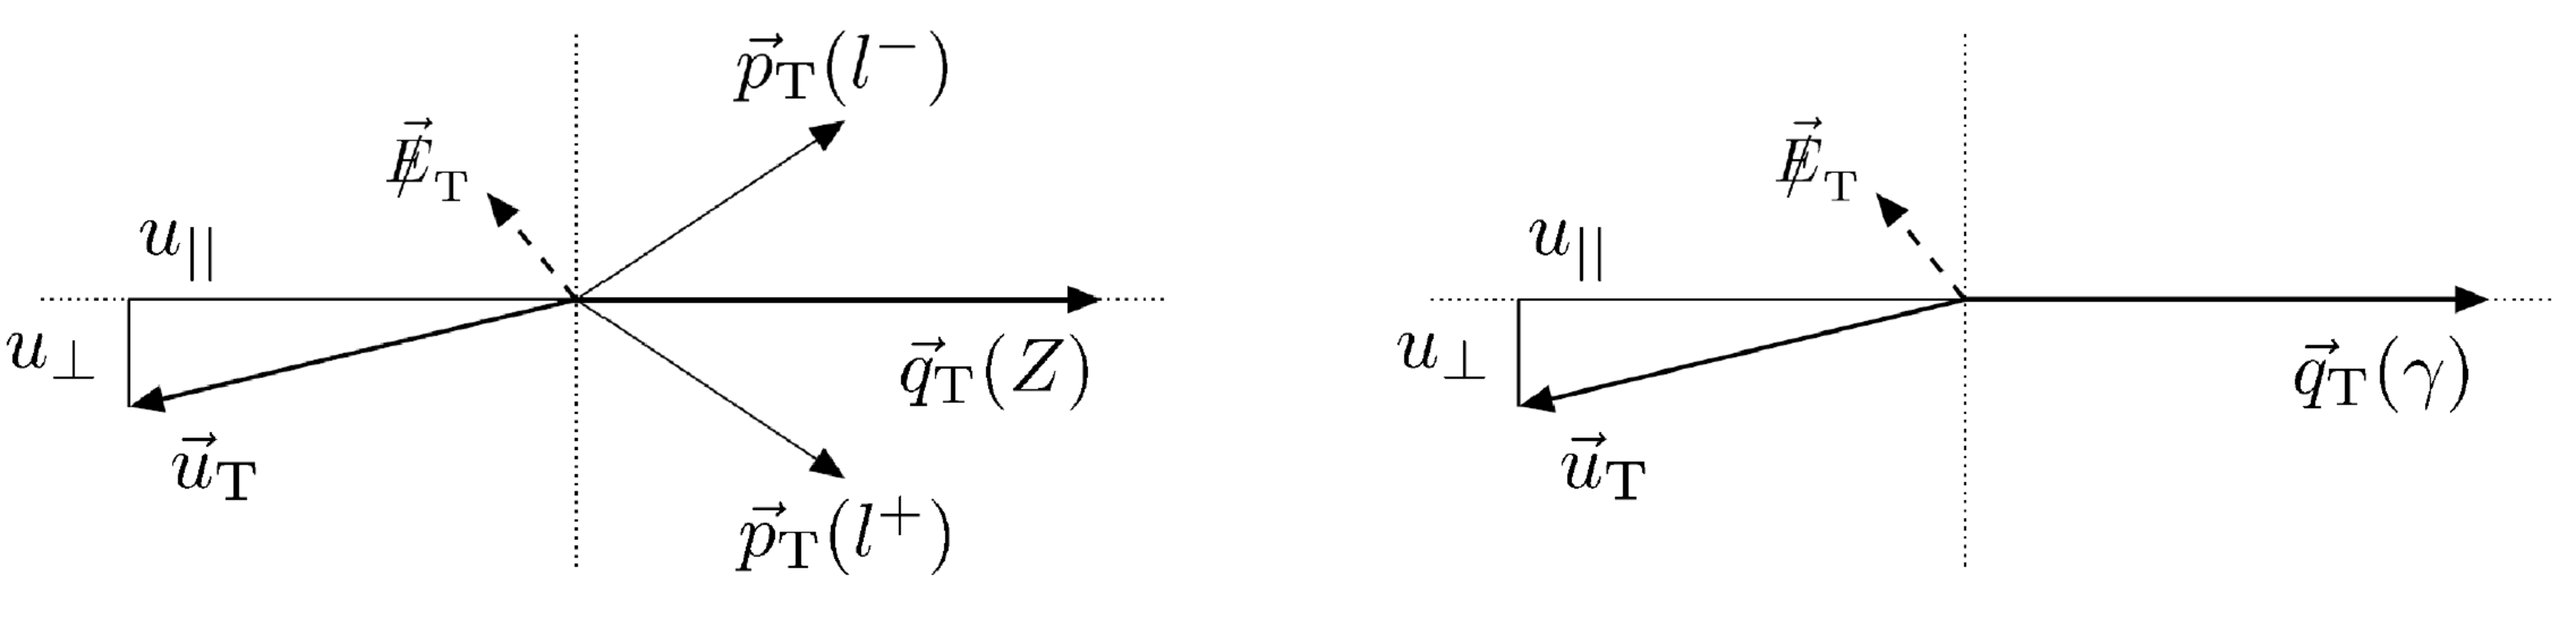
\includegraphics[width=0.8\textwidth]{images/metZgamma.pdf}
\caption{Illustration of the $\mathrm{Z\to\ell^+\ell^-}$ (left) and photon (right) event kinematics in the transverse plane.}\label{fig:metZgamma}
\end{figure}

The \MET characteristics are evaluated using two components of $\vec{u}_\mathrm{T}$, one parallel ($u_\parallel$) and one perpendicular ($u_\perp$) to the axis defined by $\vec{q}_\mathrm{T}$. The distributions of these variables are parametrized using a convolution of a Breit-Wigner and a Gaussian distribution, i.e. a Voigtian distribution, which is found to provide a good description of the observables and is used to measure the resolution in $u_\parallel$ and $u_\perp$, $\sigma(u_\parallel)$ and $\sigma(u_\perp)$, respectively. These resolutions are closely related to the \MET resolution. The resolutions $\sigma(u_\parallel)$ and $\sigma(u_\perp)$ obtained using recent 13\TeV data are shown in Fig.~\ref{fig:metres}, compared to simulations of $\mathrm{Z\to\mu^+\mu^-}$, $\mathrm{Z\to e^+ e^-}$ and $\gamma$ events.

\begin{figure}[htb]
\centering
\subfigure{
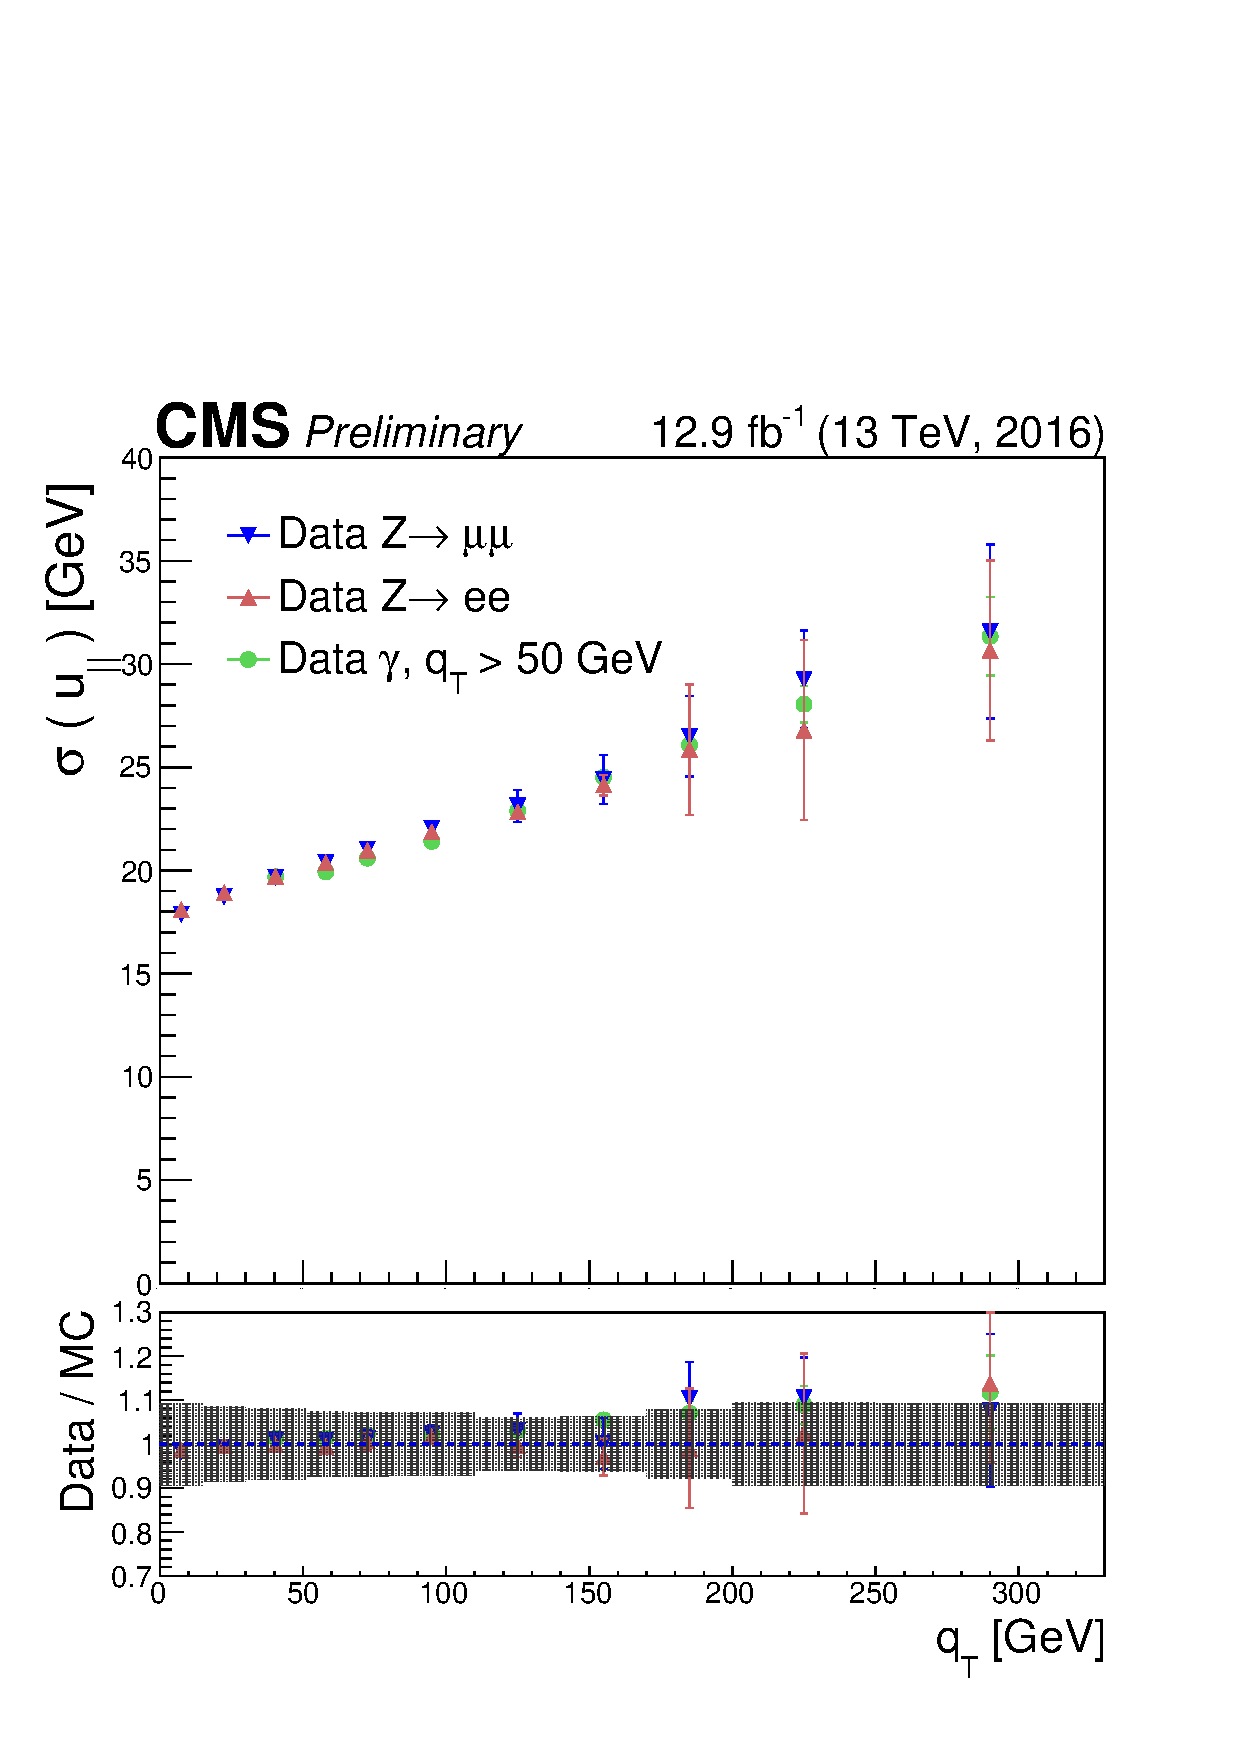
\includegraphics[width=0.45\textwidth]{images/met_parallel.pdf}
}
\subfigure{
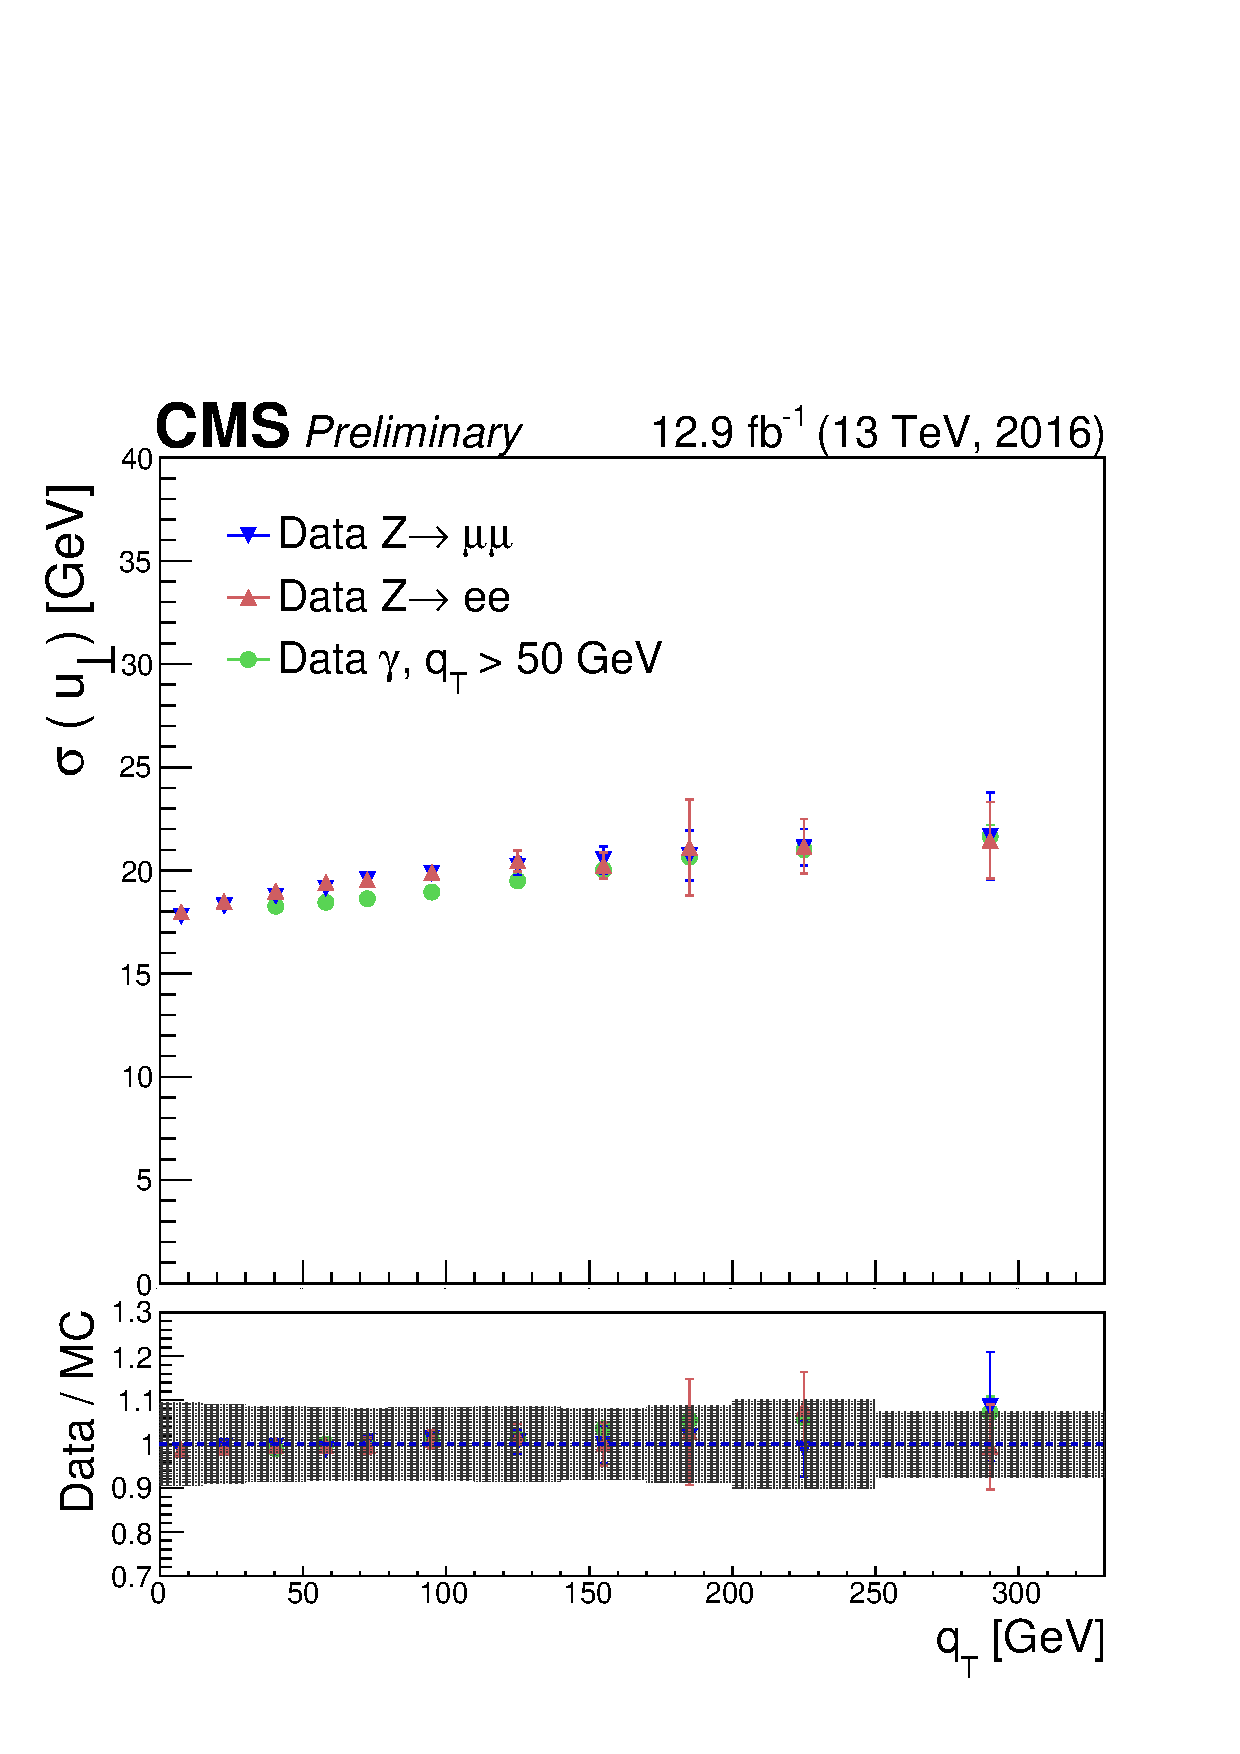
\includegraphics[width=0.45\textwidth]{images/met_perp.pdf}
}
\caption{Resolutions $\sigma(u_\parallel)$ (left) and $\sigma(u_\perp)$ (right) for $\mathrm{Z\to\mu^+\mu^-}$, $\mathrm{Z\to e^+ e^-}$ and $\gamma$ events as a function of the vector boson \pt. The upper panels show the resolution measured in data and the bottom panels the data to simulation ratio. The uncertainty band in the bottom panel represents the systematic uncertainty of the simulation, estimated as the $\mathrm{Z\to e^+ e^-}$ channel systematic uncertainty.}\label{fig:metres}
\end{figure}

